\documentclass[12pt]{article}
\usepackage[utf8]{inputenc}
\usepackage[T1]{fontenc}
\usepackage{amsmath,amssymb,amsthm}
\usepackage[margin=0.75in]{geometry}
\usepackage{hyperref}
\usepackage{booktabs}
\usepackage{tikz}
\usetikzlibrary{arrows.meta,positioning}

\hypersetup{colorlinks=true,linkcolor=blue}
\setlength{\parindent}{0pt}
\setlength{\parskip}{0.35em}
\renewcommand{\arraystretch}{1.15}

\newcommand{\problem}[1]{\vspace{0.8em}\noindent\textbf{Problem #1.}\vspace{0.35em}}
\newenvironment{solution}{\par\noindent\textit{Solution.}\ }{\par\vspace{1.1em}}
\newcommand{\subproblem}[1]{\par\vspace{0.45em}\noindent\textbf{#1}\quad}
\newcommand{\assigntext}[1]{\par\vspace{0.25em}\small\textit{#1}\par\vspace{0.35em}}

\title{Computer Systems Architecture\\Homework 4}
\author{Ashesh Kaji}
\date{}

\begin{document}
\maketitle

\problem{1}
\assigntext{In this exercise, we examine in detail how an instruction is executed in a single-cycle datapath. Problems refer to a clock cycle in which the processor fetches instruction word \texttt{0x00c6ba23}.}

\begin{solution}
Decode \texttt{0x00c6ba23}: S-type, opcode \texttt{0x23}; \texttt{funct3}=011 (\texttt{sd} in RV64). Fields: \texttt{rs1}=13, \texttt{rs2}=12, imm$=$20 (\texttt{0x14}). Semantics: \texttt{Mem[Reg[x13]+20] $\leftarrow$ Reg[x12]}.

\subproblem{1.1}
The ALU control block takes the main-control \texttt{ALUOp} field plus the \texttt{funct3}/\texttt{funct7} bits from the instruction. For loads/stores the datapath always forms \texttt{Reg[rs1]+imm}, so \texttt{ALUOp} is the ``not R-type'' encoding (e.g.\ \texttt{00} in the P\&H table) and the selected ALU op is \textbf{ADD} (output \texttt{0010} in the usual 4-bit table). Inputs: \texttt{ALUOp}$=$\texttt{00}, \texttt{funct3}$=$\texttt{011} (only used for memory width; address add is still ADD).

\subproblem{1.2}
Not a branch: next PC is \textbf{PC+4}. Path (Figure~4.21 style): PC $\rightarrow$ adder (PC+4) $\rightarrow$ input~0 of the PC mux $\rightarrow$ PC register at the next edge. Branch adder and branch \texttt{AND} are idle.

\begin{center}
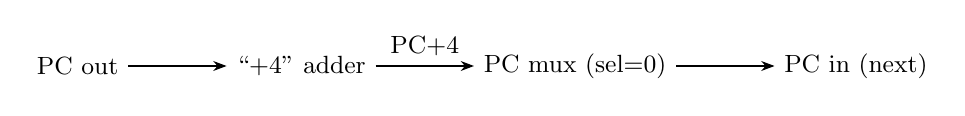
\begin{tikzpicture}[node distance=1.25cm,>=Stealth,font=\small]
  \node (pc) {PC out};
  \node[right=of pc] (a4) {``+4'' adder};
  \node[right=of a4] (mux) {PC mux (sel$=$0)};
  \node[right=of mux] (next) {PC in (next)};
  \draw[->] (pc) -- (a4);
  \draw[->] (a4) -- node[above]{PC+4} (mux);
  \draw[->] (mux) -- (next);
\end{tikzpicture}
\end{center}
If the fetched PC is $P$, new PC is $P+4$ (absolute address depends on your IMEM map; the problem only fixes the word fetched).

\subproblem{1.3}
Assume \texttt{Reg[x13]} and \texttt{Reg[x12]} are whatever your architectural state says (call them $v_{13}$, $v_{12}$). Typical muxes:
\begin{center}
\begin{tabular}{@{}llll@{}}
\toprule
Mux & Select & Inputs (conceptually) & Output \\
\midrule
PC src & 0 (not taken) & PC+4; branch target & PC+4 \\
ALU src & 1 & \texttt{rs2} ($v_{12}$); imm & imm$=$20 (sign-ext.) \\
Mem to reg & $\times$ & --- & don't care (\texttt{sd} does not write \texttt{rd}) \\
\bottomrule
\end{tabular}
\end{center}

\subproblem{1.4}
ALU: inputs $v_{13}$ and $20$ (after sign-extend/mux); op ADD; output effective address $v_{13}+20$. Adder~1 (PC+4): $P$ and $4$. Branch-target adder: not used for this opcode (inputs irrelevant / stale).

\subproblem{1.5}
Read addresses \texttt{rs1}=13, \texttt{rs2}=12; read data $v_{13}$, $v_{12}$. Write port inactive: \texttt{RegWrite}$=$0, write register/data undefined/don't-care. Control inputs to the regfile block follow main control (\texttt{sd}: no register write).
\end{solution}

\problem{2}
\assigntext{Assume the logic blocks used to implement a processor's datapath have the latencies in the table in the PDF. ``Register read'' is the time needed after the rising clock edge for the new register value to appear on the output (applies to the PC only). ``Register setup'' is the amount of time a register's data input must be stable before the rising edge (applies to both the PC and register file).}

\begin{solution}
Block delays from the PDF (ps): I/D-Mem 250; RF read 150; mux 25; ALU 200; adder 150; gate 5; PC reg read 30; reg setup 20; sign-extend 50; control 50.

\begin{center}
\begin{tabular}{@{}llllllllll@{}}
\toprule
I/D-Mem & Reg.\ file & Mux & ALU & Adder & Gate & Reg.\ read & Reg.\ setup & Sign-ext. & Control \\
\midrule
250 & 150 & 25 & 200 & 150 & 5 & 30 & 20 & 50 & 50 \\
\bottomrule
\end{tabular}
\end{center}

\subproblem{2.1}
R-type: after fetch, the RF read and control happen in parallel, then the ALU-input mux selects the second register operand, then ALU, then writeback mux/setup. So
$30+250+\max(150,50)+25+200+25+20=700$~ps.

\subproblem{2.2}
\texttt{ld}: same through ALU, then D-Mem, then \texttt{MemToReg} mux, then setup: $30+250+150+200+250+25+20 = 925$~ps. No extra mux on the load path beyond the one after memory.

\subproblem{2.3}
\texttt{sd}: no register writeback, so no final mux/setup: $30+250+150+200+250 = 880$~ps.

\subproblem{2.4}
\texttt{beq}: the branch-target adder runs in parallel with register read/sign-extend. The select signal for the PC mux comes from the compare path, so the critical path is
$30+250+\max(150,50)+25+200+5+25+20=705$~ps.

\subproblem{2.5}
I-type ALU (e.g.\ \texttt{addi}): sign-extend and control overlap with RF, so the slower side is still the RF read. Thus
$30+250+\max(150,50)+200+25+20=675$~ps.

\subproblem{2.6}
Minimum clock $=$ $\max(\cdot)=925$~ps (set by \texttt{ld}).
\end{solution}

\problem{3}
\assigntext{Part~(a) uses the instruction mix table in the PDF. Parts~(b) and~(c) refer to Figure~4.21 and Problem~2 latencies; part~(c) also uses the cost table in the PDF.}

\begin{solution}
Mix from PDF: R/I (non-\texttt{ld}) 52\%, \texttt{ld} 25\%, \texttt{sd} 11\%, \texttt{beq} 12\%. I split the 52\% evenly between R-type and I-type ALU ops (26\% each), since Problem 2 gives different latencies for those two classes.

\begin{center}
\begin{tabular}{@{}llll@{}}
\toprule
R-type / I-type (non-\texttt{ld}) & \texttt{ld} & \texttt{sd} & \texttt{beq} \\
\midrule
52\% & 25\% & 11\% & 12\% \\
\bottomrule
\end{tabular}
\end{center}

\subproblem{(a) --- per-instruction cycle time}
Suppose you could build a CPU where the clock cycle time was different for each instruction.

\subproblem{3.a1}
Average time per instruction if each type paid its own path delay:
$0.26(700)+0.26(675)+0.25(925)+0.11(880)+0.12(705)=770.15$~ps.
Fixed-period CPU is stuck at 925~ps, so speedup $925/770.15 \approx \mathbf{1.20}$.

\subproblem{(b) --- multiplier}
Consider adding a multiplier to the CPU in Figure~4.21. This adds 300~ps to the ALU latency but reduces dynamic instruction count by 5\% (no need to emulate multiply).

\subproblem{3.b1}
Without: 925~ps. With: ALU becomes 500~ps; longest path is \texttt{ld} at $30+250+150+500+250+25+20=1225$~ps.

\subproblem{3.b2}
Execution time scales as $0.95\times T_{\mathrm{clk}}$. Ratio $925/(0.95\cdot1225)\approx \mathbf{0.79}$---a slowdown, not a speedup.

\subproblem{3.b3}
Need $0.95\cdot(725+L_{\mathrm{ALU}})<925$ where $725+L$ is the \texttt{ld} path. So $L_{\mathrm{ALU}}<925/0.95-725\approx 249$~ps total ALU latency. Anything much above the original 200~ps wipes out the 5\% IC gain.

\subproblem{(c) --- more registers}
Beginning from Figure~4.21, latencies from Problem~2, and the \emph{cost} table in the PDF: suppose doubling GPRs from 32 to 64 reduces \texttt{ld} and \texttt{sd} count by 12\%, but register-file latency goes from 150~ps to 160~ps and cost doubles from 200 to 400. (Use the instruction mix from 3(a); ignore other ISA effects.)

\begin{center}
\begin{tabular}{@{}llllllllll@{}}
\toprule
I-Mem & Reg.\ file & Mux & ALU & Adder & D-Mem & Single reg. & Sign-ext. & Gate & Control \\
\midrule
1000 & 200 & 10 & 100 & 30 & 2000 & 5 & 100 & 1 & 500 \\
\bottomrule
\end{tabular}
\end{center}

\subproblem{3.c1}
Instruction count factor $0.52+0.12+0.25\cdot0.88+0.11\cdot0.88=0.9568$. Clock rises by 10~ps on every path $\Rightarrow$ 935~ps. Time ratio old/new $\approx 925/(0.9568\cdot 935)\approx \mathbf{1.03}$ (small win).

\subproblem{3.c2}
Using Figure~4.21, baseline cost is
\[
1000 + 2000 + 200 + 3(10) + 100 + 2(30) + 5 + 100 + 1 + 500 = 3996.
\]
Only the register file changes, so the new cost is $3996-200+400=4196$, i.e.\ a cost ratio of
$4196/3996 \approx 1.05$.
So performance goes up by about $3.4\%$, but total cost also goes up by about $5.0\%$. Net performance-per-cost is
$1.034/1.050 \approx 0.985$, so this is slightly worse on a value basis.

\subproblem{3.c3}
It makes sense when spill traffic is bad enough that even a small execution-time win matters more than the modest area/cost increase. It does \emph{not} make much sense if you care about performance per dollar, because here the total machine gets about $5\%$ more expensive for only about a $3\%$ speedup.
\end{solution}

\problem{4}
\assigntext{\texttt{ld} has the longest latency on the CPU from Section~4.4 (RISC-V text). If \texttt{ld}/\texttt{sd} had no immediate offset (address must already be in \texttt{rs1}), no instruction would use both ALU and data memory in one cycle, reducing clock time but often replacing one memory op with two instructions.}

\begin{solution}
\subproblem{4.1}
New \texttt{ld}/\texttt{sd} drop the ALU from the access path: \texttt{ld} becomes $30+250+150+250+25+20=725$~ps; \texttt{sd} becomes $680$~ps. Using the corrected Problem~2 timings, the new clock is
$\max(700,725,680,705,675)=725$~ps.

\subproblem{4.2}
Instruction count scales by $0.52+0.25\cdot2+0.11\cdot2+0.12=1.36$. Time $\propto 1.36\cdot 725$ vs.\ $1\cdot 925$: ratio
$\approx 1.066$---still \textbf{slower}, but only by about $6.6\%$.

\subproblem{4.3}
Whether the IC blow-up (36\% more instructions) outweighs the clock improvement (925$\to$725).

\subproblem{4.4}
Original is usually the better general-purpose design: one instruction for a simple addressing mode is worth the longer cycle. The ``split'' ISA only wins if you almost never use offsets and can tolerate extra code.
\end{solution}

\problem{5}
\assigntext{Examine adding \texttt{lwi.d rd, rs1, rs2} (``Load With Increment''): $\texttt{Reg[rd]} = \texttt{Mem[Reg[rs1] + Reg[rs2]]}$.}

\begin{solution}
\subproblem{5.a1}
None. \texttt{Reg[rs1]+Reg[rs2]} is already what the ALU does with \texttt{ALUSrc}$=$0.

\subproblem{5.a2}
Control: decode a new opcode/funct, set \texttt{MemRead}, \texttt{RegWrite}, \texttt{ALUSrc}$=$0, \texttt{MemToReg}$=$1, and the usual ALU op ADD. Possibly the immediate generator if you reuse its field encoding (then imm hardware is unused).

\subproblem{5.a3}
No new wires beyond what \texttt{ld} already needs: \texttt{rs2} already goes to the ALU bus for R-types; you need the control path to allow that combination on a load. The critical path may grow (same as \texttt{ld} today).
\end{solution}

\problem{6}
\assigntext{Pipelining and clock cycle time. Use stage latencies and the instruction breakdown from the PDF.}

\begin{solution}
Stages (PDF): IF 250, ID 350, EX 150, MEM 300, WB 200~ps. Instruction mix: ALU 45\%, branch/jump 20\%, load 20\%, store 15\%.

\begin{center}
\begin{tabular}{@{}lllll@{}}
\toprule
IF & ID & EX & MEM & WB \\
\midrule
250 & 350 & 150 & 300 & 200 \\
\bottomrule
\end{tabular}
\qquad
\begin{tabular}{@{}llll@{}}
\toprule
ALU/Logic & Jump/Branch & Load & Store \\
\midrule
45\% & 20\% & 20\% & 15\% \\
\bottomrule
\end{tabular}
\end{center}

\subproblem{6.1}
Non-pipelined: $250+350+150+300+200=1250$~ps per cycle. Pipelined: cycle $=\max=350$~ps.

\subproblem{6.2}
One \texttt{ld} still traverses all five stages: $\approx 5\cdot350=1750$~ps (pipelined) vs.\ $1250$~ps (non-pipelined) end-to-end---pipelining improves throughput, not single-instruction latency.

\subproblem{6.3}
Split the slowest stage (ID, 350~ps) into two 175~ps stages; new bottleneck is MEM at 300~ps, so clock becomes \textbf{300}~ps.

\subproblem{6.4}
Data memory used only in MEM for loads/stores: $20\%+15\%=35\%$ of cycles in steady state.

\subproblem{6.5}
WB writes on ALU ops and loads (not stores/branches): $45\%+20\%=65\%$.
\end{solution}

\problem{7}
\assigntext{What is the minimum number of cycles needed to completely execute $n$ instructions on a CPU with a $k$-stage pipeline? Justify your formula.}

\begin{solution}
Need $k$ cycles to fill the pipe and finish the first instruction, then $n-1$ more cycles for the remaining instructions: $\boxed{n+k-1}$ cycles (equivalently $k+(n-1)$). First insn occupies stages 1\ldots $k$ in successive cycles; each later insn adds one cycle at steady state. For $n=1$ this gives $k$, as expected.
\end{solution}

\problem{8}
\begin{solution}
\subproblem{(a)}
Assume \texttt{x11}$=11$ and \texttt{x12}$=22$. On a pipeline from Section~4.5 that does \emph{not} handle data hazards (programmer inserts \texttt{NOP}s as needed), what are the final values of \texttt{x13} and \texttt{x14}?
\begin{verbatim}
addi x11, x12, 5
add  x13, x11, x12
addi x14, x11, 15
\end{verbatim}
\texttt{addi} finishes WB after \texttt{add}'s ID, so \texttt{add} still reads old \texttt{x11}$=11$: \texttt{x13}$=11+22=33$. \texttt{addi x14} IDs while the first \texttt{addi} is still in MEM/EX, so again \texttt{x11}$=11$: \texttt{x14}$=11+15=26$.

\subproblem{(b)}
Same initial \texttt{x11}, \texttt{x12}. What is the final value of \texttt{x15}? Register file: written at the beginning of the cycle, read at the end; ID sees WB from the same cycle (Section~4.7, Figure~4.51).
\begin{verbatim}
addi x11, x12, 5
add  x13, x11, x12
addi x14, x11, 15
add  x15, x11, x11
\end{verbatim}
Now \texttt{add x15} IDs in the same cycle as the first \texttt{addi} WB, so both reads of \texttt{x11} see $22+5=27$: \texttt{x15}$=27+27=54$.

\subproblem{(c)}
Insert \texttt{NOP}s so the following runs correctly without hazard hardware:
\begin{verbatim}
addi x11, x12, 5
nop
nop
nop
add  x13, x11, x12
addi x14, x11, 15
nop
nop
nop
add  x15, x13, x12
\end{verbatim}
With back-to-back IF and WB five cycles later, a dependent consumer must have $\mathrm{IF}_{\mathrm{cons}}\ge \mathrm{IF}_{\mathrm{prod}}+4$. So three \texttt{nop}s after the first \texttt{addi}, and three \texttt{nop}s between \texttt{addi x14} and the final \texttt{add} (the producer \texttt{add x13} is four slots earlier).
\end{solution}

\end{document}
